\indent Acorde a lo solicitado, mostraremos los mejores y peores casos para nuestro algoritmo, y adem\'as, daremos el tiempo estimado 
seg\'un la complejidad del algoritmo calculada anteriormente.\\

Luego de chequear varios instancias, pudimos llegar a la conclusi\'on que uno de los tipos de casos que resulta m\'as beneficioso para nuestro algoritmo
es en el cual ambas ramas de la mediana se encuentran ya ordenadas\\

Para llegar a dicha conclusi\'on trabajamos con un total de 100 instancias y un n entre 1 y 1010000 obtuvimos que nuestro
algoritmo finaliza lo solicitado demorando 333 milisegundos.\\

Para una mayor observacion desarrollamos el siguiente grafico con las instancias:\\

\vspace*{0.3cm} \vspace*{0.3cm}
  \begin{center}
% 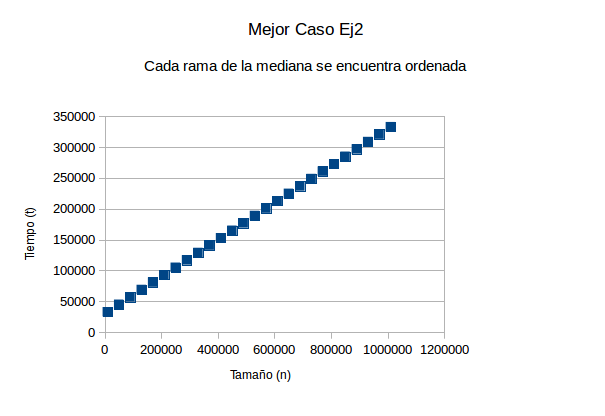
\includegraphics[scale=0.8]{./EJ2/grafico2ejmejorcaso.png}
  \end{center}
  \vspace*{0.3cm}
  
Y dividiendo por la complejidad de nuestro algoritmo llegamos a:\\

\vspace*{0.3cm} \vspace*{0.3cm}
  \begin{center}
 %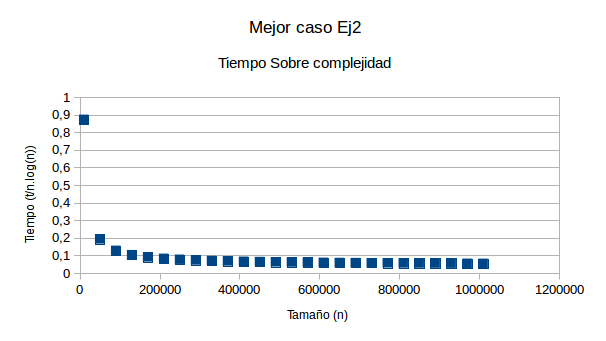
\includegraphics[scale=0.8]{./EJ2/grafico2ejmejorcaso1.png}
  \end{center}
  \vspace*{0.3cm}

Para realizar esta experimentaci\'on nos parecio prudente, realizar un promedio con el mismo input (n entre 1 y 1001000) de aproximadamente 20 corridas
tanto para la complejidad como para nuestro algoritmo y una vez calculado dicho promedio de ambas cosas realizamos la divisi\'on para
obtener resultados m\'as relevantes.\\ 

Se puede observar, como luego de realizar la divisi\'on por la complejidad cuando el n aumenta el valor tiende a 0.\\

A continuaci\'on mostraremos una tabla  con los 10 datos de medici\'on mas relevantes  y mostraremos un promedio de la totalidad de las instancias probadas.\\

\begin{table}[H]

    \begin{tabular}{ | l | l |l |}
    \hline
	Tamaño($n$) & Tiempo($t$) & \textbf{$t /n.log(n)$}  \\ \hline
730000 & 249000 & 0,058 \\ \hline
770000 & 261000 & 0,058 \\ \hline
810000 & 273000 & 0,057 \\ \hline
850000 & 285000 & 0,057 \\ \hline
890000 & 297000 & 0,056 \\ \hline
930000 & 309000 & 0,056 \\ \hline
970000 & 321000 & 0,055 \\ \hline
1010000 & 333000 & 0,055 \\ \hline
    \textbf{Promedio} & & 0,104  \\ \hline

    \end{tabular}
\end{table}

\textbf{Promedio final de todas las instancias: 0,104}\\

Verificando el peor caso, llegamos a la conclusi\'on que el tipo de caso en el que resulta menos beneficioso trabajar con nuestro algoritmo ser\'a cuando
ambas ramas se encuentran desordenadas.
\\

Realizando experimentos con un total de 100 instancias con un n variando desde 1 hasta 1010000 obtuvimos que nuestro
algoritmo, resuelve lo mencionado en 385 milisegundos, a continuaci\'on mostraremos un gr\'afico que ejemplifica lo enunciado.\\

\vspace*{0.3cm} \vspace*{0.3cm}
  \begin{center}
 %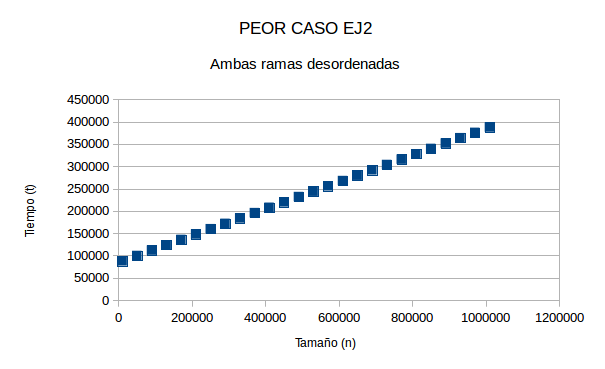
\includegraphics[scale=0.8]{./EJ2/grafico2ejpeorcaso.png}
  \end{center}
  \vspace*{0.3cm}


Y dividiendo por la complejidad propuesta llegamos a:\\

\vspace*{0.3cm} \vspace*{0.3cm}
  \begin{center}
 %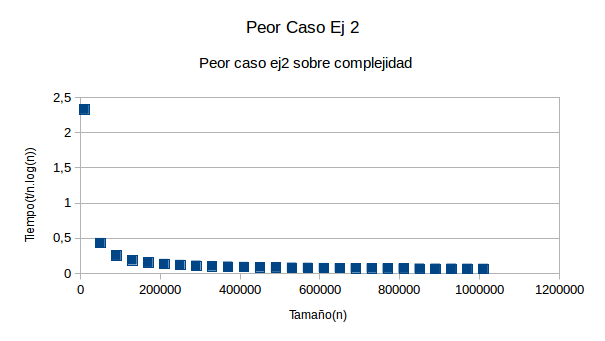
\includegraphics[scale=0.8]{./EJ2/grafico2ejpeorcaso1.png}
  \end{center}
  \vspace*{0.3cm}

Para realizar esta experimentaci\'on nos parecio acorde, realizar un promedio con el mismo input de aproximadamente 20 corridas
tanto para la complejidad como para nuestro algoritmo y una vez calculado dicho promedio de ambas cosas realizamos la divisi\'on para
obtener resultados m\'as relevantes.\\ 

Se puede observar que a pesar de tardar varios milisegundos este tipo de caso, al dividir por vuestra complejidad
es propenso a tender a 0 quedando comparativamente por encima del mejor caso.\\

A continuaci\'on mostraremos una tabla de valores de lass ultimas 10 instancias y
mostraremos el promedio total conseguido .\\


\begin{table}[H]

    \begin{tabular}{ | l | l |l |}
    \hline
Tamaño($n$) & Tiempo($t$) & \textbf{$t /n.log(n)$}  \\ \hline
610000 & 268000 & 0,076 \\ \hline
650000 & 280000 & 0,074 \\ \hline
690000 & 292000 & 0,073 \\ \hline
730000 & 304000 & 0,071 \\ \hline
770000 & 316000 & 0,070 \\ \hline
810000 & 328000 & 0,069 \\ \hline
850000 & 340000 & 0,068 \\ \hline
890000 & 352000 & 0,067 \\ \hline
930000 & 364000 & 0,066 \\ \hline
970000 & 376000 & 0,065 \\ \hline
1010000 & 388000 & 0,064 \\ \hline
    \textbf{Promedio} & & 0,195
 \\ \hline

    \end{tabular}
\end{table}

\textbf{Promedio total conseguido: 0,195}\\

Se puede observar como el peor caso presenta un promedio mayor que el mejor caso, concluyendo lo que enunciamos inicialmente.\\
